% Options for packages loaded elsewhere
\PassOptionsToPackage{unicode}{hyperref}
\PassOptionsToPackage{hyphens}{url}
\PassOptionsToPackage{dvipsnames,svgnames,x11names}{xcolor}
%
\documentclass[
]{report}

\usepackage{amsmath,amssymb}
\usepackage{lmodern}
\usepackage{iftex}
\ifPDFTeX
  \usepackage[T1]{fontenc}
  \usepackage[utf8]{inputenc}
  \usepackage{textcomp} % provide euro and other symbols
\else % if luatex or xetex
  \usepackage{unicode-math}
  \defaultfontfeatures{Scale=MatchLowercase}
  \defaultfontfeatures[\rmfamily]{Ligatures=TeX,Scale=1}
\fi
% Use upquote if available, for straight quotes in verbatim environments
\IfFileExists{upquote.sty}{\usepackage{upquote}}{}
\IfFileExists{microtype.sty}{% use microtype if available
  \usepackage[]{microtype}
  \UseMicrotypeSet[protrusion]{basicmath} % disable protrusion for tt fonts
}{}
\makeatletter
\@ifundefined{KOMAClassName}{% if non-KOMA class
  \IfFileExists{parskip.sty}{%
    \usepackage{parskip}
  }{% else
    \setlength{\parindent}{0pt}
    \setlength{\parskip}{6pt plus 2pt minus 1pt}}
}{% if KOMA class
  \KOMAoptions{parskip=half}}
\makeatother
\usepackage{xcolor}
\setlength{\emergencystretch}{3em} % prevent overfull lines
\setcounter{secnumdepth}{-\maxdimen} % remove section numbering
% Make \paragraph and \subparagraph free-standing
\ifx\paragraph\undefined\else
  \let\oldparagraph\paragraph
  \renewcommand{\paragraph}[1]{\oldparagraph{#1}\mbox{}}
\fi
\ifx\subparagraph\undefined\else
  \let\oldsubparagraph\subparagraph
  \renewcommand{\subparagraph}[1]{\oldsubparagraph{#1}\mbox{}}
\fi

\usepackage{color}
\usepackage{fancyvrb}
\newcommand{\VerbBar}{|}
\newcommand{\VERB}{\Verb[commandchars=\\\{\}]}
\DefineVerbatimEnvironment{Highlighting}{Verbatim}{commandchars=\\\{\}}
% Add ',fontsize=\small' for more characters per line
\newenvironment{Shaded}{}{}
\newcommand{\AlertTok}[1]{\textcolor[rgb]{0.58,0.85,0.30}{\textbf{\colorbox[rgb]{0.30,0.12,0.14}{#1}}}}
\newcommand{\AnnotationTok}[1]{\textcolor[rgb]{0.31,0.63,0.31}{#1}}
\newcommand{\AttributeTok}[1]{\textcolor[rgb]{0.65,0.15,0.64}{#1}}
\newcommand{\BaseNTok}[1]{\textcolor[rgb]{0.60,0.41,0.00}{#1}}
\newcommand{\BuiltInTok}[1]{\textcolor[rgb]{0.65,0.15,0.64}{#1}}
\newcommand{\CharTok}[1]{\textcolor[rgb]{0.31,0.63,0.31}{#1}}
\newcommand{\CommentTok}[1]{\textcolor[rgb]{0.63,0.63,0.65}{\textit{#1}}}
\newcommand{\CommentVarTok}[1]{\textcolor[rgb]{0.89,0.34,0.29}{\textit{#1}}}
\newcommand{\ConstantTok}[1]{\textcolor[rgb]{0.60,0.41,0.00}{#1}}
\newcommand{\ControlFlowTok}[1]{\textcolor[rgb]{0.65,0.15,0.64}{#1}}
\newcommand{\DataTypeTok}[1]{\textcolor[rgb]{0.65,0.15,0.64}{#1}}
\newcommand{\DecValTok}[1]{\textcolor[rgb]{0.60,0.41,0.00}{#1}}
\newcommand{\DocumentationTok}[1]{\textcolor[rgb]{0.89,0.34,0.29}{#1}}
\newcommand{\ErrorTok}[1]{\textcolor[rgb]{0.96,0.28,0.28}{\underline{#1}}}
\newcommand{\ExtensionTok}[1]{\textcolor[rgb]{0.25,0.47,0.95}{\textbf{#1}}}
\newcommand{\FloatTok}[1]{\textcolor[rgb]{0.60,0.41,0.00}{#1}}
\newcommand{\FunctionTok}[1]{\textcolor[rgb]{0.25,0.47,0.95}{#1}}
\newcommand{\ImportTok}[1]{\textcolor[rgb]{0.31,0.63,0.31}{#1}}
\newcommand{\InformationTok}[1]{\textcolor[rgb]{0.77,0.36,0.00}{#1}}
\newcommand{\KeywordTok}[1]{\textcolor[rgb]{0.65,0.15,0.64}{#1}}
\newcommand{\NormalTok}[1]{\textcolor[rgb]{0.22,0.23,0.26}{#1}}
\newcommand{\OperatorTok}[1]{\textcolor[rgb]{0.65,0.15,0.64}{#1}}
\newcommand{\OtherTok}[1]{\textcolor[rgb]{0.15,0.68,0.38}{#1}}
\newcommand{\PreprocessorTok}[1]{\textcolor[rgb]{0.65,0.15,0.64}{#1}}
\newcommand{\RegionMarkerTok}[1]{\textcolor[rgb]{0.16,0.50,0.73}{\colorbox[rgb]{0.08,0.19,0.26}{#1}}}
\newcommand{\SpecialCharTok}[1]{\textcolor[rgb]{0.00,0.52,0.74}{#1}}
\newcommand{\SpecialStringTok}[1]{\textcolor[rgb]{0.85,0.27,0.33}{#1}}
\newcommand{\StringTok}[1]{\textcolor[rgb]{0.31,0.63,0.31}{#1}}
\newcommand{\VariableTok}[1]{\textcolor[rgb]{0.89,0.34,0.29}{#1}}
\newcommand{\VerbatimStringTok}[1]{\textcolor[rgb]{0.85,0.27,0.33}{#1}}
\newcommand{\WarningTok}[1]{\textcolor[rgb]{0.85,0.27,0.33}{#1}}

\providecommand{\tightlist}{%
  \setlength{\itemsep}{0pt}\setlength{\parskip}{0pt}}\usepackage{longtable,booktabs,array}
\usepackage{calc} % for calculating minipage widths
% Correct order of tables after \paragraph or \subparagraph
\usepackage{etoolbox}
\makeatletter
\patchcmd\longtable{\par}{\if@noskipsec\mbox{}\fi\par}{}{}
\makeatother
% Allow footnotes in longtable head/foot
\IfFileExists{footnotehyper.sty}{\usepackage{footnotehyper}}{\usepackage{footnote}}
\makesavenoteenv{longtable}
\usepackage{graphicx}
\makeatletter
\def\maxwidth{\ifdim\Gin@nat@width>\linewidth\linewidth\else\Gin@nat@width\fi}
\def\maxheight{\ifdim\Gin@nat@height>\textheight\textheight\else\Gin@nat@height\fi}
\makeatother
% Scale images if necessary, so that they will not overflow the page
% margins by default, and it is still possible to overwrite the defaults
% using explicit options in \includegraphics[width, height, ...]{}
\setkeys{Gin}{width=\maxwidth,height=\maxheight,keepaspectratio}
% Set default figure placement to htbp
\makeatletter
\def\fps@figure{htbp}
\makeatother

\makeatletter
\makeatother
\makeatletter
\makeatother
\makeatletter
\@ifpackageloaded{caption}{}{\usepackage{caption}}
\AtBeginDocument{%
\ifdefined\contentsname
  \renewcommand*\contentsname{Table of contents}
\else
  \newcommand\contentsname{Table of contents}
\fi
\ifdefined\listfigurename
  \renewcommand*\listfigurename{List of Figures}
\else
  \newcommand\listfigurename{List of Figures}
\fi
\ifdefined\listtablename
  \renewcommand*\listtablename{List of Tables}
\else
  \newcommand\listtablename{List of Tables}
\fi
\ifdefined\figurename
  \renewcommand*\figurename{Figure}
\else
  \newcommand\figurename{Figure}
\fi
\ifdefined\tablename
  \renewcommand*\tablename{Table}
\else
  \newcommand\tablename{Table}
\fi
}
\@ifpackageloaded{float}{}{\usepackage{float}}
\floatstyle{ruled}
\@ifundefined{c@chapter}{\newfloat{codelisting}{h}{lop}}{\newfloat{codelisting}{h}{lop}[chapter]}
\floatname{codelisting}{Listing}
\newcommand*\listoflistings{\listof{codelisting}{List of Listings}}
\makeatother
\makeatletter
\@ifpackageloaded{caption}{}{\usepackage{caption}}
\@ifpackageloaded{subcaption}{}{\usepackage{subcaption}}
\makeatother
\makeatletter
\@ifpackageloaded{tcolorbox}{}{\usepackage[many]{tcolorbox}}
\makeatother
\makeatletter
\@ifundefined{shadecolor}{\definecolor{shadecolor}{rgb}{.97, .97, .97}}
\makeatother
\makeatletter
\makeatother
\ifLuaTeX
  \usepackage{selnolig}  % disable illegal ligatures
\fi
\IfFileExists{bookmark.sty}{\usepackage{bookmark}}{\usepackage{hyperref}}
\IfFileExists{xurl.sty}{\usepackage{xurl}}{} % add URL line breaks if available
\urlstyle{same} % disable monospaced font for URLs
\hypersetup{
  pdftitle={Graffiti Impact on Crimes},
  pdfauthor={Linh Tran},
  colorlinks=true,
  linkcolor={blue},
  filecolor={Maroon},
  citecolor={Blue},
  urlcolor={Blue},
  pdfcreator={LaTeX via pandoc}}

\title{Graffiti Impact on Crimes}
\usepackage{etoolbox}
\makeatletter
\providecommand{\subtitle}[1]{% add subtitle to \maketitle
  \apptocmd{\@title}{\par {\large #1 \par}}{}{}
}
\makeatother
\subtitle{An explanatory analysis on the relationship between Graffiti
Removal and Crime Rates in the City of Chicago}
\author{Linh Tran}
\date{6/3/23}

\begin{document}
\maketitle
\ifdefined\Shaded\renewenvironment{Shaded}{\begin{tcolorbox}[breakable, borderline west={3pt}{0pt}{shadecolor}, enhanced, frame hidden, interior hidden, sharp corners, boxrule=0pt]}{\end{tcolorbox}}\fi

\renewcommand*\contentsname{Table of contents}
{
\hypersetup{linkcolor=}
\setcounter{tocdepth}{2}
\tableofcontents
}
\hypertarget{introduction}{%
\section{Introduction}\label{introduction}}

The City of Chicago, with a population of about 2.7 million people, is
one of the most popular cities in the United States, known for its
vibrant and diverse neighborhoods (Data USA, 2020). However, Chicago has
also gained attention for its crime rate, which has been a persistent
challenge for the city. The issue of crime in Chicago has been a complex
and multifaceted challenge, with various factors contributing to its
prevalence. Graffiti has been an agonizing issue in urban areas, posing
challenges to cities in terms of aesthetics, safety, and community
well-being. As a result, I have conducted an analysis to study the
relationship between graffiti removal and the crime rate in the City of
Chicago, focusing specifically on \textbf{criminal crimes} and the years
from \textbf{2016 to 2018} (most recent pre-COVID time to attain an
understanding of the situation in normal circumstances).

This report aims to provide insights into the potential linkages between
graffiti removal efforts and crime rates in Chicago. By analyzing and
interpreting relevant data, we can gain a better understanding of how
graffiti removal efforts may impact crime rates and inform strategies
for addressing this issue in the city. This report will delve into the
data findings, highlighting patterns and trends, and drawing
evidence-based conclusions to shed light on the relationship between
graffiti removal and crime rate in the City of Chicago.

\hypertarget{important-findings}{%
\section{Important Findings}\label{important-findings}}

\hypertarget{a-quick-glance}{%
\subsection{A quick glance}\label{a-quick-glance}}

The graph below is a side-by-side comparison of the average crime rate
and graffiti removal request rate in the 77 community areas of Chicago.

\begin{Shaded}
\begin{Highlighting}[]
\NormalTok{p1 }\OtherTok{=} \FunctionTok{ggplot}\NormalTok{() }\SpecialCharTok{+}
  \FunctionTok{geom\_polygon}\NormalTok{(}\AttributeTok{data=}\NormalTok{comm\_map, }\AttributeTok{mapping=}\FunctionTok{aes}\NormalTok{(}\AttributeTok{x=}\NormalTok{long, }\AttributeTok{y=}\NormalTok{lat, }\AttributeTok{group=}\NormalTok{group, }\AttributeTok{fill=}\NormalTok{avg\_crime\_rate)) }\SpecialCharTok{+}
  \FunctionTok{geom\_path}\NormalTok{(}\AttributeTok{data=}\NormalTok{comm\_map, }\AttributeTok{mapping=}\FunctionTok{aes}\NormalTok{(}\AttributeTok{x=}\NormalTok{long, }\AttributeTok{y=}\NormalTok{lat, }\AttributeTok{group=}\NormalTok{group), }\AttributeTok{color=}\StringTok{"gray90"}\NormalTok{,}\AttributeTok{linewidth=}\FloatTok{0.2}\NormalTok{) }\SpecialCharTok{+}
  \FunctionTok{scale\_fill\_gradient}\NormalTok{(}\AttributeTok{low=}\StringTok{"\#ffffb2"}\NormalTok{, }\AttributeTok{high=}\StringTok{"\#bd0026"}\NormalTok{,}
                      \AttributeTok{name=}\StringTok{"Reported Incidents}\SpecialCharTok{\textbackslash{}n}\StringTok{per 100 Residents"}\NormalTok{,}
                      \AttributeTok{limits=}\FunctionTok{c}\NormalTok{(}\DecValTok{0}\NormalTok{,}\DecValTok{40}\NormalTok{),}
                      \AttributeTok{breaks=}\FunctionTok{c}\NormalTok{(}\DecValTok{0}\NormalTok{,}\DecValTok{10}\NormalTok{,}\DecValTok{20}\NormalTok{,}\DecValTok{30}\NormalTok{,}\DecValTok{40}\NormalTok{)) }\SpecialCharTok{+}
  \FunctionTok{geom\_path}\NormalTok{(}\AttributeTok{data=}\NormalTok{central\_map, }\AttributeTok{mapping=}\FunctionTok{aes}\NormalTok{(}\AttributeTok{x=}\NormalTok{long, }\AttributeTok{y=}\NormalTok{lat, }\AttributeTok{group=}\NormalTok{group), }\AttributeTok{color=}\StringTok{\textquotesingle{}grey50\textquotesingle{}}\NormalTok{)}\SpecialCharTok{+}
  \FunctionTok{coord\_quickmap}\NormalTok{() }\SpecialCharTok{+}
  \FunctionTok{theme\_map}\NormalTok{() }\SpecialCharTok{+}
  \FunctionTok{annotate}\NormalTok{(}\AttributeTok{geom=}\StringTok{"curve"}\NormalTok{, }\AttributeTok{x=}\SpecialCharTok{{-}}\FloatTok{87.61}\NormalTok{, }\AttributeTok{xend=} \SpecialCharTok{{-}}\FloatTok{87.58}\NormalTok{, }\AttributeTok{y=}\FloatTok{41.9}\NormalTok{, }\AttributeTok{yend=}\FloatTok{41.93}\NormalTok{,}
           \AttributeTok{curvature =} \SpecialCharTok{{-}}\NormalTok{.}\DecValTok{4}\NormalTok{, }\AttributeTok{arrow=}\FunctionTok{arrow}\NormalTok{(}\AttributeTok{length=}\FunctionTok{unit}\NormalTok{(}\DecValTok{1}\NormalTok{,}\StringTok{"mm"}\NormalTok{)), }\AttributeTok{color=}\StringTok{\textquotesingle{}grey50\textquotesingle{}}\NormalTok{) }\SpecialCharTok{+}
  \FunctionTok{annotate}\NormalTok{(}\AttributeTok{geom=}\StringTok{"text"}\NormalTok{,}\AttributeTok{x=}\SpecialCharTok{{-}}\FloatTok{87.549}\NormalTok{, }\AttributeTok{y=}\FloatTok{41.937}\NormalTok{, }\AttributeTok{label =} \StringTok{"Central Business}\SpecialCharTok{\textbackslash{}n}\StringTok{District"}\NormalTok{,}
           \AttributeTok{size =} \FloatTok{2.5}\NormalTok{, }\AttributeTok{color=}\StringTok{\textquotesingle{}grey30\textquotesingle{}}\NormalTok{) }\SpecialCharTok{+}
  \FunctionTok{annotate}\NormalTok{(}\AttributeTok{geom=}\StringTok{"curve"}\NormalTok{, }\AttributeTok{x=}\SpecialCharTok{{-}}\FloatTok{87.929}\NormalTok{, }\AttributeTok{xend=} \SpecialCharTok{{-}}\FloatTok{87.92}\NormalTok{, }\AttributeTok{y=}\FloatTok{41.956}\NormalTok{, }\AttributeTok{yend=}\FloatTok{41.9417}\NormalTok{,}
           \AttributeTok{curvature =}\NormalTok{ .}\DecValTok{3}\NormalTok{, }\AttributeTok{arrow=}\FunctionTok{arrow}\NormalTok{(}\AttributeTok{length=}\FunctionTok{unit}\NormalTok{(}\DecValTok{1}\NormalTok{,}\StringTok{"mm"}\NormalTok{)), }\AttributeTok{color=}\StringTok{\textquotesingle{}grey50\textquotesingle{}}\NormalTok{) }\SpecialCharTok{+}
  \FunctionTok{annotate}\NormalTok{(}\AttributeTok{geom=}\StringTok{"text"}\NormalTok{,}\AttributeTok{x=}\SpecialCharTok{{-}}\FloatTok{87.9}\NormalTok{, }\AttributeTok{y=}\FloatTok{41.93}\NormalTok{, }\AttributeTok{label =} \StringTok{"Chicago O\textquotesingle{}Hare}\SpecialCharTok{\textbackslash{}n}\StringTok{International Airport"}\NormalTok{,}
           \AttributeTok{size =} \FloatTok{2.5}\NormalTok{, }\AttributeTok{color=}\StringTok{\textquotesingle{}grey30\textquotesingle{}}\NormalTok{) }\SpecialCharTok{+}
  \FunctionTok{guides}\NormalTok{(}\AttributeTok{fill =} \FunctionTok{guide\_colourbar}\NormalTok{(}\AttributeTok{barwidth =} \DecValTok{1}\NormalTok{, }\AttributeTok{barheight=}\DecValTok{8}\NormalTok{))}\SpecialCharTok{+}
  \FunctionTok{labs}\NormalTok{(}\AttributeTok{title=}\StringTok{"Average Criminal Crime Rate}\SpecialCharTok{\textbackslash{}n}\StringTok{in 2016{-}2018 by Community Area in Chicago"}\NormalTok{) }\SpecialCharTok{+}
  \FunctionTok{theme}\NormalTok{(}\AttributeTok{legend.position=}\FunctionTok{c}\NormalTok{(}\FloatTok{0.05}\NormalTok{,}\FloatTok{0.15}\NormalTok{), }
        \AttributeTok{legend.background =} \FunctionTok{element\_rect}\NormalTok{(}\AttributeTok{fill=}\StringTok{"transparent"}\NormalTok{),}
        \AttributeTok{legend.title =} \FunctionTok{element\_text}\NormalTok{(}\AttributeTok{size=}\DecValTok{8}\NormalTok{, }\AttributeTok{vjust=}\FloatTok{1.05}\NormalTok{, }\AttributeTok{color=}\StringTok{\textquotesingle{}grey30\textquotesingle{}}\NormalTok{),}
        \AttributeTok{legend.text =} \FunctionTok{element\_text}\NormalTok{(}\AttributeTok{color=}\StringTok{\textquotesingle{}grey40\textquotesingle{}}\NormalTok{),}
        \AttributeTok{plot.title =} \FunctionTok{element\_text}\NormalTok{(}\AttributeTok{size=}\DecValTok{10}\NormalTok{))}


\NormalTok{p2 }\OtherTok{=} \FunctionTok{ggplot}\NormalTok{() }\SpecialCharTok{+}
  \FunctionTok{geom\_polygon}\NormalTok{(}\AttributeTok{data=}\NormalTok{comm\_map, }\AttributeTok{mapping=}\FunctionTok{aes}\NormalTok{(}\AttributeTok{x=}\NormalTok{long, }\AttributeTok{y=}\NormalTok{lat, }\AttributeTok{group=}\NormalTok{group, }\AttributeTok{fill=}\NormalTok{graffiti\_requests\_per\_100)) }\SpecialCharTok{+}
  \FunctionTok{geom\_path}\NormalTok{(}\AttributeTok{data=}\NormalTok{comm\_map, }\AttributeTok{mapping=}\FunctionTok{aes}\NormalTok{(}\AttributeTok{x=}\NormalTok{long, }\AttributeTok{y=}\NormalTok{lat, }\AttributeTok{group=}\NormalTok{group), }\AttributeTok{color=}\StringTok{"gray90"}\NormalTok{,}\AttributeTok{linewidth=}\FloatTok{0.2}\NormalTok{) }\SpecialCharTok{+}
  \FunctionTok{scale\_fill\_gradient}\NormalTok{(}\AttributeTok{low=}\StringTok{"\#BBFCF1"}\NormalTok{, }\AttributeTok{high=}\StringTok{"\#122C69"}\NormalTok{,}
                      \AttributeTok{name=}\StringTok{"Number of Requests}\SpecialCharTok{\textbackslash{}n}\StringTok{per 100 Residents"}\NormalTok{,}
                      \AttributeTok{limits=}\FunctionTok{c}\NormalTok{(}\DecValTok{0}\NormalTok{,}\DecValTok{80}\NormalTok{),}
                      \AttributeTok{breaks=}\FunctionTok{c}\NormalTok{(}\DecValTok{0}\NormalTok{,}\DecValTok{20}\NormalTok{,}\DecValTok{40}\NormalTok{,}\DecValTok{60}\NormalTok{,}\DecValTok{80}\NormalTok{)) }\SpecialCharTok{+}
  \FunctionTok{geom\_path}\NormalTok{(}\AttributeTok{data=}\NormalTok{central\_map, }\AttributeTok{mapping=}\FunctionTok{aes}\NormalTok{(}\AttributeTok{x=}\NormalTok{long, }\AttributeTok{y=}\NormalTok{lat, }\AttributeTok{group=}\NormalTok{group), }\AttributeTok{color=}\StringTok{\textquotesingle{}grey60\textquotesingle{}}\NormalTok{)}\SpecialCharTok{+}
  \FunctionTok{coord\_quickmap}\NormalTok{() }\SpecialCharTok{+}
  \FunctionTok{theme\_map}\NormalTok{() }\SpecialCharTok{+}
  \FunctionTok{annotate}\NormalTok{(}\AttributeTok{geom=}\StringTok{"curve"}\NormalTok{, }\AttributeTok{x=}\SpecialCharTok{{-}}\FloatTok{87.61}\NormalTok{, }\AttributeTok{xend=} \SpecialCharTok{{-}}\FloatTok{87.58}\NormalTok{, }\AttributeTok{y=}\FloatTok{41.9}\NormalTok{, }\AttributeTok{yend=}\FloatTok{41.93}\NormalTok{,}
           \AttributeTok{curvature =} \SpecialCharTok{{-}}\NormalTok{.}\DecValTok{4}\NormalTok{, }\AttributeTok{arrow=}\FunctionTok{arrow}\NormalTok{(}\AttributeTok{length=}\FunctionTok{unit}\NormalTok{(}\DecValTok{1}\NormalTok{,}\StringTok{"mm"}\NormalTok{)), }\AttributeTok{color=}\StringTok{\textquotesingle{}grey50\textquotesingle{}}\NormalTok{) }\SpecialCharTok{+}
  \FunctionTok{annotate}\NormalTok{(}\AttributeTok{geom=}\StringTok{"text"}\NormalTok{,}\AttributeTok{x=}\SpecialCharTok{{-}}\FloatTok{87.549}\NormalTok{, }\AttributeTok{y=}\FloatTok{41.937}\NormalTok{, }\AttributeTok{label =} \StringTok{"Central Business}\SpecialCharTok{\textbackslash{}n}\StringTok{District"}\NormalTok{,}
           \AttributeTok{size =} \FloatTok{2.5}\NormalTok{, }\AttributeTok{color=}\StringTok{\textquotesingle{}grey30\textquotesingle{}}\NormalTok{) }\SpecialCharTok{+}
  \FunctionTok{annotate}\NormalTok{(}\AttributeTok{geom=}\StringTok{"curve"}\NormalTok{, }\AttributeTok{x=}\SpecialCharTok{{-}}\FloatTok{87.929}\NormalTok{, }\AttributeTok{xend=} \SpecialCharTok{{-}}\FloatTok{87.92}\NormalTok{, }\AttributeTok{y=}\FloatTok{41.956}\NormalTok{, }\AttributeTok{yend=}\FloatTok{41.9417}\NormalTok{,}
           \AttributeTok{curvature =}\NormalTok{ .}\DecValTok{3}\NormalTok{, }\AttributeTok{arrow=}\FunctionTok{arrow}\NormalTok{(}\AttributeTok{length=}\FunctionTok{unit}\NormalTok{(}\DecValTok{1}\NormalTok{,}\StringTok{"mm"}\NormalTok{)), }\AttributeTok{color=}\StringTok{\textquotesingle{}grey50\textquotesingle{}}\NormalTok{) }\SpecialCharTok{+}
  \FunctionTok{annotate}\NormalTok{(}\AttributeTok{geom=}\StringTok{"text"}\NormalTok{,}\AttributeTok{x=}\SpecialCharTok{{-}}\FloatTok{87.9}\NormalTok{, }\AttributeTok{y=}\FloatTok{41.93}\NormalTok{, }\AttributeTok{label =} \StringTok{"Chicago O\textquotesingle{}Hare}\SpecialCharTok{\textbackslash{}n}\StringTok{International Airport"}\NormalTok{,}
           \AttributeTok{size =} \FloatTok{2.5}\NormalTok{, }\AttributeTok{color=}\StringTok{\textquotesingle{}grey30\textquotesingle{}}\NormalTok{) }\SpecialCharTok{+}
  \FunctionTok{guides}\NormalTok{(}\AttributeTok{fill =} \FunctionTok{guide\_colourbar}\NormalTok{(}\AttributeTok{barwidth =} \DecValTok{1}\NormalTok{, }\AttributeTok{barheight=}\DecValTok{8}\NormalTok{))}\SpecialCharTok{+}
  \FunctionTok{labs}\NormalTok{(}\AttributeTok{title=}\StringTok{"Average Rate of Graffiti Removal Requests}\SpecialCharTok{\textbackslash{}n}\StringTok{in 2016{-}2018 by Community Area in Chicago"}\NormalTok{)}\SpecialCharTok{+}
  \FunctionTok{theme}\NormalTok{(}\AttributeTok{legend.position=}\FunctionTok{c}\NormalTok{(}\FloatTok{0.05}\NormalTok{,}\FloatTok{0.15}\NormalTok{), }
        \AttributeTok{legend.background =} \FunctionTok{element\_rect}\NormalTok{(}\AttributeTok{fill=}\StringTok{"transparent"}\NormalTok{),}
        \AttributeTok{legend.title =} \FunctionTok{element\_text}\NormalTok{(}\AttributeTok{size=}\DecValTok{8}\NormalTok{, }\AttributeTok{vjust=}\FloatTok{1.05}\NormalTok{, }\AttributeTok{color=}\StringTok{\textquotesingle{}grey30\textquotesingle{}}\NormalTok{),}
        \AttributeTok{legend.text =} \FunctionTok{element\_text}\NormalTok{(}\AttributeTok{color=}\StringTok{\textquotesingle{}grey40\textquotesingle{}}\NormalTok{),}
        \AttributeTok{plot.title =} \FunctionTok{element\_text}\NormalTok{(}\AttributeTok{size=}\DecValTok{10}\NormalTok{))}


\FunctionTok{grid.arrange}\NormalTok{(p1, p2, }\AttributeTok{nrow=}\DecValTok{1}\NormalTok{,}
             \AttributeTok{bottom=}\FunctionTok{text\_grob}\NormalTok{(}\StringTok{"Source: Chicago Data Portal \& Chicago Metropolitan Agency for Planning"}\NormalTok{, }\AttributeTok{size=}\DecValTok{10}\NormalTok{, }\AttributeTok{color=}\StringTok{\textquotesingle{}grey40\textquotesingle{}}\NormalTok{))}
\end{Highlighting}
\end{Shaded}

\begin{figure}[H]

\caption{Figure 1: Quick glance at Chicago's 77 community areas}

{\centering 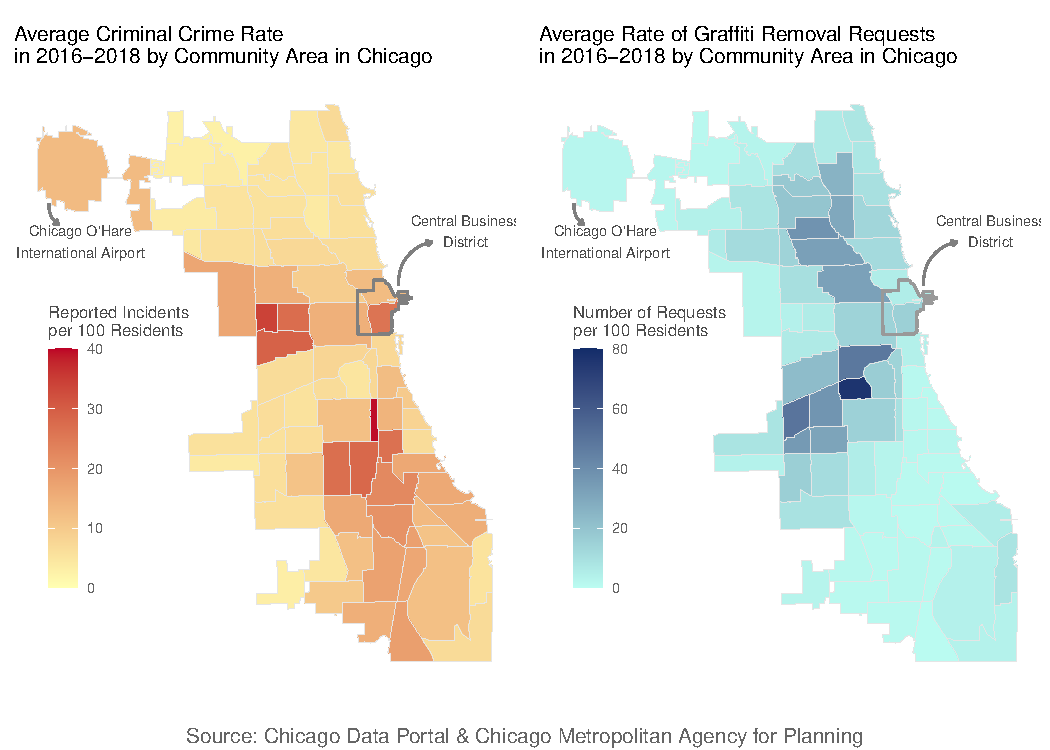
\includegraphics{final_solo_files/figure-pdf/unnamed-chunk-2-1.pdf}

}

\end{figure}

The graph shows a contrasting relationship between the crime rate and
graffiti removal request rate. That is, areas with more crimes tend to
have fewer requests (per 100 residents) and vice versa. For example, the
south area is one where this relationship is quite pronounced as it has
a very high crime rate and a low number of graffiti removal requests.
Overall, the relationship is not 100\% clear on this map as there are
areas where the crime rate and the request rate are both low (e.g.~the
far north area), but further discovery will be discussed in the sections
below.

\hypertarget{criminal-damage-crimes-and-other-criminal-crimes}{%
\subsection{Criminal Damage Crimes and Other Criminal
Crimes}\label{criminal-damage-crimes-and-other-criminal-crimes}}

One may argue that the number of graffiti removal requests in an area
would depend on its level of criminal damage crime rate -- that is,
areas with more vandalism and similar incidents should have more
graffiti, hence more removal requests than those with fewer graffiti. In
this specific case, however, this is neither entirely true nor wrong.

\begin{Shaded}
\begin{Highlighting}[]
\NormalTok{community\_crime\_adj }\OtherTok{=}\NormalTok{ community\_crime }\SpecialCharTok{|\textgreater{}} 
  \FunctionTok{arrange}\NormalTok{(graffiti\_requests\_per\_100)}

\FunctionTok{ggplot}\NormalTok{(community\_crime\_adj, }\FunctionTok{aes}\NormalTok{(}\AttributeTok{x=}\NormalTok{avg\_crim\_dam\_rate, }\AttributeTok{y=}\NormalTok{avg\_non\_dam\_crime\_rate, }\AttributeTok{color=}\NormalTok{graffiti\_requests\_per\_100)) }\SpecialCharTok{+}
  \FunctionTok{geom\_point}\NormalTok{(}\AttributeTok{size=}\FloatTok{3.5}\NormalTok{, }\AttributeTok{alpha=}\FloatTok{0.8}\NormalTok{) }\SpecialCharTok{+}
  \FunctionTok{theme\_minimal}\NormalTok{() }\SpecialCharTok{+}
  \FunctionTok{scale\_color\_gradient}\NormalTok{(}\StringTok{"Number of Requests}\SpecialCharTok{\textbackslash{}n}\StringTok{per 100 Residents"}\NormalTok{,}
                       \AttributeTok{low=}\StringTok{"\#BBFCF1"}\NormalTok{, }\AttributeTok{high=}\StringTok{"\#122C69"}\NormalTok{,}
                       \AttributeTok{limits =} \FunctionTok{c}\NormalTok{(}\DecValTok{0}\NormalTok{,}\DecValTok{80}\NormalTok{),}
                       \AttributeTok{breaks=}\NormalTok{scales}\SpecialCharTok{::}\FunctionTok{pretty\_breaks}\NormalTok{(}\AttributeTok{n=}\DecValTok{5}\NormalTok{))}\SpecialCharTok{+}
  \FunctionTok{scale\_y\_continuous}\NormalTok{(}\AttributeTok{breaks=}\NormalTok{scales}\SpecialCharTok{::}\FunctionTok{pretty\_breaks}\NormalTok{(}\AttributeTok{n=}\DecValTok{6}\NormalTok{),}
                     \AttributeTok{limit=}\FunctionTok{c}\NormalTok{(}\DecValTok{0}\NormalTok{,}\DecValTok{40}\NormalTok{))}\SpecialCharTok{+}
  \FunctionTok{scale\_x\_continuous}\NormalTok{(}\AttributeTok{limit=}\FunctionTok{c}\NormalTok{(}\DecValTok{0}\NormalTok{,}\DecValTok{5}\NormalTok{))}\SpecialCharTok{+}
  \FunctionTok{guides}\NormalTok{(}\AttributeTok{colour =} \FunctionTok{guide\_colourbar}\NormalTok{(}\AttributeTok{barwidth =} \DecValTok{10}\NormalTok{, }\AttributeTok{barheight=}\DecValTok{1}\NormalTok{, }\AttributeTok{direction =} \StringTok{"horizontal"}\NormalTok{)) }\SpecialCharTok{+}
  \FunctionTok{theme}\NormalTok{(}\AttributeTok{legend.position =} \StringTok{\textquotesingle{}bottom\textquotesingle{}}\NormalTok{,}
        \AttributeTok{legend.title =} \FunctionTok{element\_text}\NormalTok{(}\AttributeTok{size=}\DecValTok{9}\NormalTok{, }\AttributeTok{vjust=}\FloatTok{1.05}\NormalTok{, }\AttributeTok{color=}\StringTok{\textquotesingle{}grey40\textquotesingle{}}\NormalTok{),}
        \AttributeTok{legend.text =} \FunctionTok{element\_text}\NormalTok{(}\AttributeTok{color=}\StringTok{\textquotesingle{}grey40\textquotesingle{}}\NormalTok{),}
        \AttributeTok{axis.title =} \FunctionTok{element\_text}\NormalTok{(}\AttributeTok{color=}\StringTok{\textquotesingle{}grey30\textquotesingle{}}\NormalTok{, }\AttributeTok{size=}\DecValTok{11}\NormalTok{),}
        \AttributeTok{plot.subtitle =} \FunctionTok{element\_text}\NormalTok{(}\AttributeTok{color=}\StringTok{\textquotesingle{}grey20\textquotesingle{}}\NormalTok{),}
        \AttributeTok{plot.caption =} \FunctionTok{element\_text}\NormalTok{(}\AttributeTok{color=}\StringTok{\textquotesingle{}grey30\textquotesingle{}}\NormalTok{)) }\SpecialCharTok{+}
  \FunctionTok{labs}\NormalTok{(}\AttributeTok{title =} \StringTok{"Criminal Damage Crimes Rate vs. Other Crimes Rate}\SpecialCharTok{\textbackslash{}n}\StringTok{by Community Area in Chicago 2016{-}2018"}\NormalTok{,}
       \AttributeTok{subtitle=}\StringTok{"Areas with higher criminal damage crime rate tend to also have higher rate}\SpecialCharTok{\textbackslash{}n}\StringTok{for other crimes. Areas with the most number of graffiti removal requests}\SpecialCharTok{\textbackslash{}n}\StringTok{are those of lower crime rates."}\NormalTok{,}
       \AttributeTok{caption=}\StringTok{"Source: Chicago Data Portal \& Chicago Metropolitan Agency for Planning"}\NormalTok{,}
       \AttributeTok{x=}\StringTok{"Average Rate of Criminal Damage Crimes (\%)"}\NormalTok{,}
       \AttributeTok{y=}\StringTok{"Average Rate of Other Criminal Crimes (\%)"}\NormalTok{)}\SpecialCharTok{+}
  \FunctionTok{annotate}\NormalTok{(}\StringTok{"rect"}\NormalTok{, }\AttributeTok{xmin=}\FloatTok{0.2}\NormalTok{, }\AttributeTok{xmax=}\FloatTok{1.5}\NormalTok{, }\AttributeTok{ymin=}\FloatTok{0.2}\NormalTok{, }\AttributeTok{ymax=}\DecValTok{15}\NormalTok{, }\AttributeTok{alpha=}\FloatTok{0.07}\NormalTok{)}
\end{Highlighting}
\end{Shaded}

\begin{figure}[H]

\caption{Figure 2: Graffiti Removal and Criminal Damage Crimes vs.~Other
Crimes}

{\centering 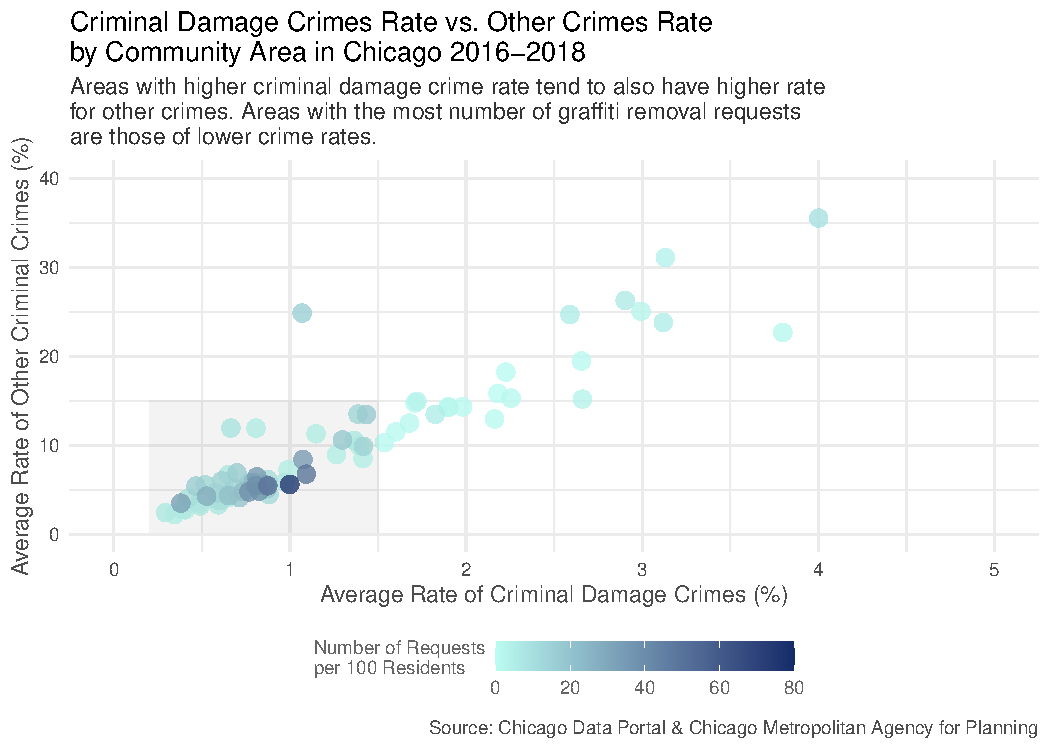
\includegraphics{final_solo_files/figure-pdf/unnamed-chunk-3-1.pdf}

}

\end{figure}

This graph illustrates that areas with very high crime rates (either
criminal damage or other criminal crimes) still have very few graffiti
removal requests. Assuming that the criminal damage crime rate (which
includes vandalism) is somewhat representative of graffiti incidents,
this would imply that the low number of graffiti requests in high
crime-level areas is not because these areas do not have any graffiti to
remove, but simply because they do not do so.

However, the question remains in the lower crime level areas: there is
still a mixture of both high and low numbers of graffiti removal
requests in the shaded area (low crime rate) in the graph above and it
is shown more clearly in the graph below:

\begin{Shaded}
\begin{Highlighting}[]
\FunctionTok{ggplot}\NormalTok{(community\_crime, }\FunctionTok{aes}\NormalTok{(}\AttributeTok{x=}\NormalTok{graffiti\_requests\_per\_100, }\AttributeTok{fill=}\NormalTok{crime\_level))}\SpecialCharTok{+}
  \FunctionTok{geom\_density}\NormalTok{(}\AttributeTok{alpha=}\FloatTok{0.4}\NormalTok{) }\SpecialCharTok{+}
  \FunctionTok{theme\_minimal}\NormalTok{() }\SpecialCharTok{+}
  \FunctionTok{theme}\NormalTok{(}\AttributeTok{legend.position =} \FunctionTok{c}\NormalTok{(}\FloatTok{0.8}\NormalTok{, }\FloatTok{0.8}\NormalTok{),}
        \AttributeTok{legend.text =} \FunctionTok{element\_text}\NormalTok{(}\AttributeTok{color=}\StringTok{\textquotesingle{}grey40\textquotesingle{}}\NormalTok{),}
        \AttributeTok{legend.title =} \FunctionTok{element\_text}\NormalTok{(}\AttributeTok{color=}\StringTok{\textquotesingle{}grey40\textquotesingle{}}\NormalTok{, }\AttributeTok{size=}\DecValTok{10}\NormalTok{),}
        \AttributeTok{axis.title.y =} \FunctionTok{element\_blank}\NormalTok{(),}
        \AttributeTok{axis.text.y =} \FunctionTok{element\_blank}\NormalTok{(),}
        \AttributeTok{axis.title.x =} \FunctionTok{element\_text}\NormalTok{(}\AttributeTok{color=}\StringTok{\textquotesingle{}grey30\textquotesingle{}}\NormalTok{, }\AttributeTok{size=}\DecValTok{11}\NormalTok{),}
        \AttributeTok{plot.caption =} \FunctionTok{element\_text}\NormalTok{(}\AttributeTok{color=}\StringTok{\textquotesingle{}grey30\textquotesingle{}}\NormalTok{)) }\SpecialCharTok{+}
  \FunctionTok{labs}\NormalTok{(}\AttributeTok{x=}\StringTok{"Number of Graffiti Removal Requests}\SpecialCharTok{\textbackslash{}n}\StringTok{per 100 Residents"}\NormalTok{,}
       \AttributeTok{fill=}\StringTok{"Crime Level"}\NormalTok{,}
       \AttributeTok{caption=}\StringTok{"Source: Chicago Data Portal \& Chicago Metropolitan Agency for Planning"}\NormalTok{) }\SpecialCharTok{+}
  \FunctionTok{annotate}\NormalTok{(}\AttributeTok{geom=}\StringTok{"text"}\NormalTok{, }\AttributeTok{x=}\DecValTok{20}\NormalTok{, }\AttributeTok{y=}\FloatTok{0.06}\NormalTok{, }\AttributeTok{size =} \DecValTok{4}\NormalTok{,}\AttributeTok{color=}\StringTok{\textquotesingle{}grey40\textquotesingle{}}\NormalTok{,}
           \AttributeTok{label=}\StringTok{"Low crime level areas generally have more requests,}\SpecialCharTok{\textbackslash{}n}\StringTok{except for these areas, where they have}\SpecialCharTok{\textbackslash{}n}\StringTok{few requests yet low crime rates"}\NormalTok{, }\AttributeTok{hjust=}\DecValTok{0}\NormalTok{)}\SpecialCharTok{+}
  \FunctionTok{annotate}\NormalTok{(}\StringTok{"rect"}\NormalTok{, }\AttributeTok{xmin=}\DecValTok{0}\NormalTok{, }\AttributeTok{xmax=}\DecValTok{15}\NormalTok{, }\AttributeTok{ymin=}\DecValTok{0}\NormalTok{, }\AttributeTok{ymax=}\FloatTok{0.04}\NormalTok{, }\AttributeTok{alpha=}\FloatTok{0.2}\NormalTok{) }\SpecialCharTok{+}
  \FunctionTok{annotate}\NormalTok{(}\AttributeTok{geom=}\StringTok{"curve"}\NormalTok{, }\AttributeTok{x=}\DecValTok{18}\NormalTok{, }\AttributeTok{xend=} \DecValTok{11}\NormalTok{, }\AttributeTok{y=}\FloatTok{0.06}\NormalTok{, }\AttributeTok{yend=}\FloatTok{0.045}\NormalTok{,}
           \AttributeTok{curvature =}\NormalTok{ .}\DecValTok{3}\NormalTok{, }\AttributeTok{arrow=}\FunctionTok{arrow}\NormalTok{(}\AttributeTok{length=}\FunctionTok{unit}\NormalTok{(}\DecValTok{1}\NormalTok{,}\StringTok{"mm"}\NormalTok{)), }\AttributeTok{color=}\StringTok{\textquotesingle{}grey60\textquotesingle{}}\NormalTok{)}
\end{Highlighting}
\end{Shaded}

\begin{figure}[H]

\caption{Figure 3: The Distribution of Graffiti Removal Request Rate by
Crime Level}

{\centering 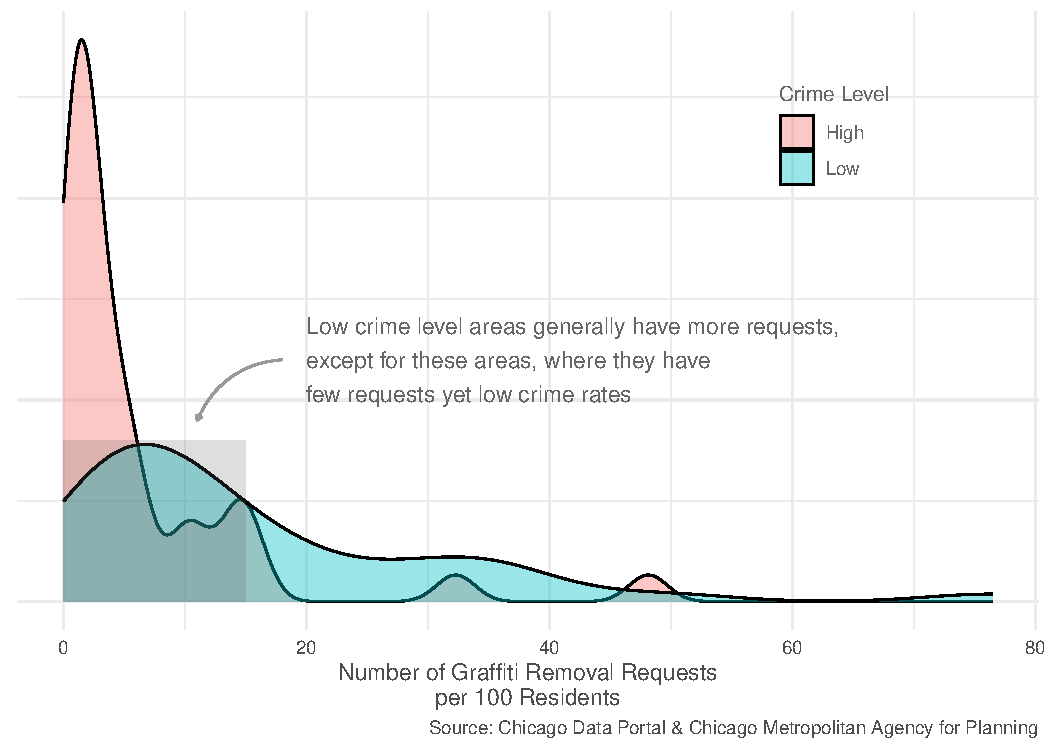
\includegraphics{final_solo_files/figure-pdf/unnamed-chunk-4-1.pdf}

}

\end{figure}

\hypertarget{income-plays-an-important-role}{%
\subsection{Income Plays an Important
Role}\label{income-plays-an-important-role}}

One possible explanation for the observation in question above is that
areas of higher levels of income generally have lower crime rates, or
fewer graffiti vandalism incidents, hence reducing the need to submit a
graffiti removal request.

\begin{Shaded}
\begin{Highlighting}[]
\FunctionTok{ggplot}\NormalTok{(community\_crime, }\FunctionTok{aes}\NormalTok{(}\AttributeTok{x=}\NormalTok{graffiti\_requests\_per\_100, }\AttributeTok{y=}\NormalTok{avg\_crime\_rate, }\AttributeTok{color=}\NormalTok{inc\_level)) }\SpecialCharTok{+}
  \FunctionTok{geom\_point}\NormalTok{(}\AttributeTok{size =} \FloatTok{2.5}\NormalTok{, }\AttributeTok{alpha=}\FloatTok{0.8}\NormalTok{) }\SpecialCharTok{+}
  \FunctionTok{theme\_minimal}\NormalTok{()}\SpecialCharTok{+}
  \FunctionTok{gghighlight}\NormalTok{(}\AttributeTok{unhighlighted\_params =} \FunctionTok{list}\NormalTok{(}\AttributeTok{alpha=}\FloatTok{0.3}\NormalTok{)) }\SpecialCharTok{+} 
  \FunctionTok{facet\_wrap}\NormalTok{(}\FunctionTok{vars}\NormalTok{(inc\_level)) }\SpecialCharTok{+}
  \FunctionTok{scale\_color\_manual}\NormalTok{(}\AttributeTok{values =} \FunctionTok{c}\NormalTok{(}\StringTok{"\#BDAAD5"}\NormalTok{, }\StringTok{"\#9882B1"}\NormalTok{, }\StringTok{"\#7c668d"}\NormalTok{)) }\SpecialCharTok{+}
  \FunctionTok{labs}\NormalTok{(}\AttributeTok{x=}\StringTok{"Number of Graffiti Removal Requests}\SpecialCharTok{\textbackslash{}n}\StringTok{per 100 Residents"}\NormalTok{,}
       \AttributeTok{y=}\StringTok{"Average Overall Crime Rate (\%)"}\NormalTok{,}
       \AttributeTok{caption=}\StringTok{"Source: Chicago Data Portal \& Chicago Metropolitan Agency for Planning"}\NormalTok{,}
       \AttributeTok{title =} \StringTok{"Effect of Income on the Relationship between}\SpecialCharTok{\textbackslash{}n}\StringTok{Graffiti Removal and Average Crime Rate"}\NormalTok{,}
       \AttributeTok{subtitle =} \StringTok{"The relationship is more pronounced in areas wherein income is low to medium.}\SpecialCharTok{\textbackslash{}n}\StringTok{Wealthy areas typically have lower crime rate, thus fewer graffiti to remove"}\NormalTok{)}\SpecialCharTok{+}
  \FunctionTok{theme}\NormalTok{(}\AttributeTok{axis.title =} \FunctionTok{element\_text}\NormalTok{(}\AttributeTok{color=}\StringTok{\textquotesingle{}grey30\textquotesingle{}}\NormalTok{, }\AttributeTok{size=}\DecValTok{10}\NormalTok{),}
        \AttributeTok{axis.title.x =} \FunctionTok{element\_text}\NormalTok{(}\AttributeTok{vjust =} \SpecialCharTok{{-}}\FloatTok{0.05}\NormalTok{),}
        \AttributeTok{plot.subtitle =} \FunctionTok{element\_text}\NormalTok{(}\AttributeTok{color=}\StringTok{\textquotesingle{}grey20\textquotesingle{}}\NormalTok{),}
        \AttributeTok{plot.caption =} \FunctionTok{element\_text}\NormalTok{(}\AttributeTok{color=}\StringTok{\textquotesingle{}grey30\textquotesingle{}}\NormalTok{, }\AttributeTok{vjust =} \SpecialCharTok{{-}}\FloatTok{0.05}\NormalTok{))}
\end{Highlighting}
\end{Shaded}

\begin{figure}[H]

\caption{Figure 4: The Impact of Income on the Relationship between
Graffiti Removal and Crime Rate}

{\centering 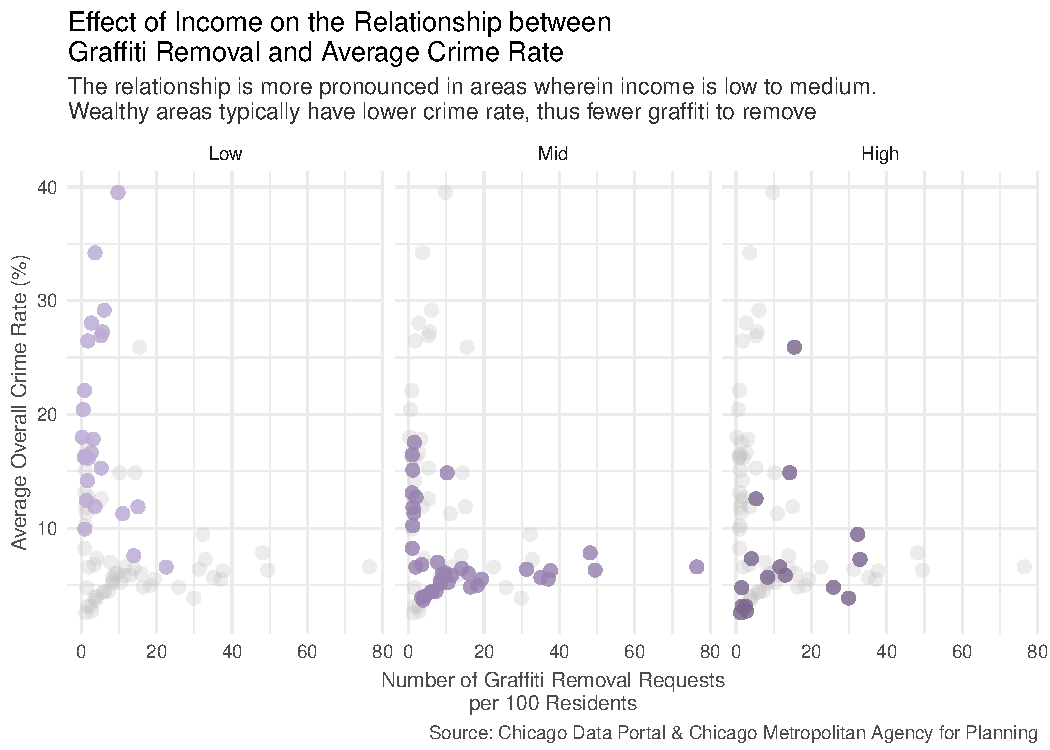
\includegraphics{final_solo_files/figure-pdf/unnamed-chunk-5-1.pdf}

}

\end{figure}

The inverse relationship between graffiti removal and crime rate is
quite clear in areas of low to medium income levels and less so for
higher-income areas. Other factors may contribute to this relationship
as well that might create some deviation from the main trend, but
overall, graffiti removal, to some extent, appears to help with crime
reduction.

\hypertarget{key-takeaway}{%
\section{Key Takeaway}\label{key-takeaway}}

Graffiti seems to be closely tied to an increase in crime incidents, and
removing graffiti is demonstrated to potentially have an impact on
reducing the crime rate. One proposed explanation for this phenomenon is
the idea of crime as an epidemic, as described by Gladwell (2002):

\begin{quote}
\emph{It says that crime is contagious---just as a fashion trend is
contagious---that it can start with a broken window and spread to an
entire community. The Tipping Point in this epidemic, though, isn't a
particular kind of person---a Connector like Lois Weisberg or a Maven
like Mark Alpert. It's something physical like graffiti. The impetus to
engage in a certain kind of behavior is not coming from a certain kind
of person but from a feature of the environment (p.141).}
\end{quote}

From this theory, it is suggested that the surroundings are crucial in
human behavior and decision-making, thus raising the importance of
maintaining a clean environment in the battle against crimes, including
removing graffiti.

Through this report, I hope to contribute to the ongoing discussions and
efforts of city officials, law enforcement agencies, and community
organizations in addressing graffiti vandalism and its potential impact
on crime rates. By examining the data and providing evidence-based
insights, this report aims to provide valuable information that can
inform decision-making and support effective strategies to mitigate
graffiti vandalism and the overall crime rate in the City of Chicago

\hypertarget{references}{%
\section{References}\label{references}}

\emph{Chicago, IL}. Data USA. (n.d.). Retrieved April 23, 2023, from
https://datausa.io/profile/geo/chicago-il

Gladwell, M. (2002). \emph{The Tipping Point: How Little Things Can Make
A Big Difference} (1st Back Bay pbk. ed). Back Bay Books

\hypertarget{code}{%
\section{Code}\label{code}}

This section is solely dedicated to demonstrate the code for data
wrangling from the raw data to the one used to create the graphs in this
report.

\begin{Shaded}
\begin{Highlighting}[]
\DocumentationTok{\#\# Download the raw data (crime data)}
\NormalTok{crime }\OtherTok{=} \FunctionTok{read\_csv}\NormalTok{(}\StringTok{\textquotesingle{}https://data.cityofchicago.org/api/views/ijzp{-}q8t2/rows.csv?accessType=DOWNLOAD\textquotesingle{}}\NormalTok{)}

\DocumentationTok{\#\# Select columns of interest and years 2016{-}2018}
\NormalTok{crime\_adj }\OtherTok{=}\NormalTok{ crime }\SpecialCharTok{|\textgreater{}} 
  \FunctionTok{select}\NormalTok{(}\FunctionTok{c}\NormalTok{(ID, Date, }\StringTok{\textasciigrave{}}\AttributeTok{Primary Type}\StringTok{\textasciigrave{}}\NormalTok{, Description, }\StringTok{\textasciigrave{}}\AttributeTok{Location Description}\StringTok{\textasciigrave{}}\NormalTok{, }\StringTok{\textasciigrave{}}\AttributeTok{Community Area}\StringTok{\textasciigrave{}}\NormalTok{, Year)) }\SpecialCharTok{|\textgreater{}} 
  \FunctionTok{filter}\NormalTok{(Year }\SpecialCharTok{\textgreater{}} \DecValTok{2015} \SpecialCharTok{\&}\NormalTok{ Year }\SpecialCharTok{\textless{}} \DecValTok{2019}\NormalTok{)}

\DocumentationTok{\#\# Focus on only criminal crimes}
\DocumentationTok{\#\# and fix name of type "Crim Sexual Assault"}
\NormalTok{criminal }\OtherTok{=}\NormalTok{ crime\_adj }\SpecialCharTok{|\textgreater{}} 
  \FunctionTok{filter}\NormalTok{(}\SpecialCharTok{!}\StringTok{\textasciigrave{}}\AttributeTok{Primary Type}\StringTok{\textasciigrave{}} \SpecialCharTok{\%in\%} \FunctionTok{c}\NormalTok{(}\StringTok{"NON {-} CRIMINAL"}\NormalTok{, }\StringTok{"NON{-}CRIMINAL"}\NormalTok{, }\StringTok{"NON{-}CRIMINAL (SUBJECT SPECIFIED)"}\NormalTok{)) }\SpecialCharTok{|\textgreater{}} 
  \FunctionTok{mutate}\NormalTok{(}\StringTok{\textasciigrave{}}\AttributeTok{Primary Type}\StringTok{\textasciigrave{}} \OtherTok{=} \FunctionTok{if\_else}\NormalTok{(}\StringTok{\textasciigrave{}}\AttributeTok{Primary Type}\StringTok{\textasciigrave{}} \SpecialCharTok{==} \StringTok{"CRIM SEXUAL ASSAULT"}\NormalTok{, }\StringTok{"CRIMINAL SEXUAL ASSAULT"}\NormalTok{, }\StringTok{\textasciigrave{}}\AttributeTok{Primary Type}\StringTok{\textasciigrave{}}\NormalTok{),}
         \StringTok{\textasciigrave{}}\AttributeTok{Community Area}\StringTok{\textasciigrave{}} \OtherTok{=} \FunctionTok{as.character}\NormalTok{(}\StringTok{\textasciigrave{}}\AttributeTok{Community Area}\StringTok{\textasciigrave{}}\NormalTok{))}

\DocumentationTok{\#\# Download raw data on graffiti removal requests}
\NormalTok{graffiti }\OtherTok{=} \FunctionTok{read\_csv}\NormalTok{(}\StringTok{"https://data.cityofchicago.org/api/views/8tus{-}apua/rows.csv?accessType=DOWNLOAD"}\NormalTok{)}

\DocumentationTok{\#\# Select columns of interest}
\NormalTok{graffiti }\OtherTok{=}\NormalTok{ graffiti }\SpecialCharTok{|\textgreater{}} 
  \FunctionTok{select}\NormalTok{(}\FunctionTok{c}\NormalTok{(}\StringTok{\textasciigrave{}}\AttributeTok{Creation Date}\StringTok{\textasciigrave{}}\NormalTok{, Status, }\StringTok{\textasciigrave{}}\AttributeTok{Completion Date}\StringTok{\textasciigrave{}}\NormalTok{, }\StringTok{\textasciigrave{}}\AttributeTok{Community Area}\StringTok{\textasciigrave{}}\NormalTok{))}

\DocumentationTok{\#\# Demographics data on community areas}
\DocumentationTok{\#\# data available at https://www.cmap.illinois.gov/data/data{-}hub}
\NormalTok{community }\OtherTok{=} \FunctionTok{read\_csv}\NormalTok{(}\StringTok{"data/cds\_202207/cds\_202207/ReferenceCCAProfiles20162020.csv"}\NormalTok{) }\SpecialCharTok{|\textgreater{}} 
  \FunctionTok{select}\NormalTok{(}\FunctionTok{c}\NormalTok{(GEOID, GEOG, TOT\_POP, MED\_AGE, UNEMP, NOT\_IN\_LBFRC, }
\NormalTok{           LT\_HS, HS, SOME\_COLL, BACH, GRAD\_PROF,}
\NormalTok{           INC\_LT\_25K, MEDINC)) }\SpecialCharTok{|\textgreater{}} 
  \FunctionTok{mutate}\NormalTok{(}\AttributeTok{GEOID =} \FunctionTok{as.character}\NormalTok{(GEOID),}
         \AttributeTok{UNEMP =} \DecValTok{100}\SpecialCharTok{*}\NormalTok{UNEMP}\SpecialCharTok{/}\NormalTok{TOT\_POP,}
         \AttributeTok{NOT\_IN\_LBFRC =} \DecValTok{100}\SpecialCharTok{*}\NormalTok{NOT\_IN\_LBFRC}\SpecialCharTok{/}\NormalTok{TOT\_POP,}
         \AttributeTok{LT\_HS =} \DecValTok{100}\SpecialCharTok{*}\NormalTok{LT\_HS}\SpecialCharTok{/}\NormalTok{TOT\_POP,}
         \AttributeTok{HS =} \DecValTok{100}\SpecialCharTok{*}\NormalTok{HS}\SpecialCharTok{/}\NormalTok{TOT\_POP,}
         \AttributeTok{SOME\_COLL =} \DecValTok{100}\SpecialCharTok{*}\NormalTok{SOME\_COLL}\SpecialCharTok{/}\NormalTok{TOT\_POP,}
         \AttributeTok{BACH =} \DecValTok{100}\SpecialCharTok{*}\NormalTok{BACH}\SpecialCharTok{/}\NormalTok{TOT\_POP,}
         \AttributeTok{GRAD\_PROF =} \DecValTok{100}\SpecialCharTok{*}\NormalTok{GRAD\_PROF}\SpecialCharTok{/}\NormalTok{TOT\_POP,}
         \AttributeTok{INC\_LT\_25K =} \DecValTok{100}\SpecialCharTok{*}\NormalTok{INC\_LT\_25K}\SpecialCharTok{/}\NormalTok{TOT\_POP)}

\DocumentationTok{\#\# Crime by Community Area}
\NormalTok{non\_dam\_crime\_rate }\OtherTok{=}\NormalTok{ criminal }\SpecialCharTok{|\textgreater{}} 
  \FunctionTok{filter}\NormalTok{(}\StringTok{\textasciigrave{}}\AttributeTok{Primary Type}\StringTok{\textasciigrave{}} \SpecialCharTok{!=} \StringTok{"CRIMINAL DAMAGE"}\NormalTok{) }\SpecialCharTok{|\textgreater{}} 
  \FunctionTok{group\_by}\NormalTok{(Year, }\StringTok{\textasciigrave{}}\AttributeTok{Community Area}\StringTok{\textasciigrave{}}\NormalTok{) }\SpecialCharTok{|\textgreater{}} 
  \FunctionTok{summarise}\NormalTok{(}\AttributeTok{total\_incidents =} \FunctionTok{n}\NormalTok{()) }\SpecialCharTok{|\textgreater{}} 
  \FunctionTok{ungroup}\NormalTok{() }\SpecialCharTok{|\textgreater{}} 
  \FunctionTok{left\_join}\NormalTok{(community, }\AttributeTok{by=}\FunctionTok{c}\NormalTok{(}\StringTok{"Community Area"} \OtherTok{=} \StringTok{"GEOID"}\NormalTok{)) }\SpecialCharTok{|\textgreater{}} 
  \FunctionTok{mutate}\NormalTok{(}\AttributeTok{crime\_rate =} \DecValTok{100}\SpecialCharTok{*}\NormalTok{total\_incidents}\SpecialCharTok{/}\NormalTok{TOT\_POP) }\SpecialCharTok{|\textgreater{}} 
  \FunctionTok{group\_by}\NormalTok{(}\FunctionTok{across}\NormalTok{(}\SpecialCharTok{{-}}\FunctionTok{c}\NormalTok{(Year,total\_incidents, crime\_rate))) }\SpecialCharTok{|\textgreater{}} 
  \FunctionTok{summarise}\NormalTok{(}\AttributeTok{avg\_non\_dam\_crime\_rate =} \FunctionTok{mean}\NormalTok{(crime\_rate))}

\NormalTok{crim\_dam\_rate }\OtherTok{=}\NormalTok{ criminal }\SpecialCharTok{|\textgreater{}} 
  \FunctionTok{filter}\NormalTok{(}\StringTok{\textasciigrave{}}\AttributeTok{Primary Type}\StringTok{\textasciigrave{}} \SpecialCharTok{==} \StringTok{"CRIMINAL DAMAGE"}\NormalTok{) }\SpecialCharTok{|\textgreater{}} 
  \FunctionTok{group\_by}\NormalTok{(Year, }\StringTok{\textasciigrave{}}\AttributeTok{Community Area}\StringTok{\textasciigrave{}}\NormalTok{) }\SpecialCharTok{|\textgreater{}} 
  \FunctionTok{summarise}\NormalTok{(}\AttributeTok{total\_incidents =} \FunctionTok{n}\NormalTok{()) }\SpecialCharTok{|\textgreater{}} 
  \FunctionTok{ungroup}\NormalTok{() }\SpecialCharTok{|\textgreater{}} 
  \FunctionTok{left\_join}\NormalTok{(community, }\AttributeTok{by=}\FunctionTok{c}\NormalTok{(}\StringTok{"Community Area"} \OtherTok{=} \StringTok{"GEOID"}\NormalTok{)) }\SpecialCharTok{|\textgreater{}} 
  \FunctionTok{mutate}\NormalTok{(}\AttributeTok{crime\_rate =} \DecValTok{100}\SpecialCharTok{*}\NormalTok{total\_incidents}\SpecialCharTok{/}\NormalTok{TOT\_POP) }\SpecialCharTok{|\textgreater{}} 
  \FunctionTok{group\_by}\NormalTok{(}\StringTok{\textasciigrave{}}\AttributeTok{Community Area}\StringTok{\textasciigrave{}}\NormalTok{) }\SpecialCharTok{|\textgreater{}} 
  \FunctionTok{summarise}\NormalTok{(}\AttributeTok{avg\_crim\_dam\_rate =} \FunctionTok{mean}\NormalTok{(crime\_rate))}
  
\DocumentationTok{\#\# Completed graffiti removal requests by Community Area}
\NormalTok{graffiti\_summary }\OtherTok{=}\NormalTok{ graffiti }\SpecialCharTok{|\textgreater{}} 
  \FunctionTok{mutate}\NormalTok{(}\StringTok{\textasciigrave{}}\AttributeTok{Creation Date}\StringTok{\textasciigrave{}} \OtherTok{=} \FunctionTok{mdy}\NormalTok{(}\StringTok{\textasciigrave{}}\AttributeTok{Creation Date}\StringTok{\textasciigrave{}}\NormalTok{),}
         \AttributeTok{year =} \FunctionTok{year}\NormalTok{(}\StringTok{\textasciigrave{}}\AttributeTok{Creation Date}\StringTok{\textasciigrave{}}\NormalTok{),}
         \StringTok{\textasciigrave{}}\AttributeTok{Community Area}\StringTok{\textasciigrave{}} \OtherTok{=} \FunctionTok{as.character}\NormalTok{(}\StringTok{\textasciigrave{}}\AttributeTok{Community Area}\StringTok{\textasciigrave{}}\NormalTok{)) }\SpecialCharTok{|\textgreater{}} 
  \FunctionTok{filter}\NormalTok{(year }\SpecialCharTok{\textless{}} \DecValTok{2019} \SpecialCharTok{\&}\NormalTok{ year }\SpecialCharTok{\textgreater{}} \DecValTok{2015}\NormalTok{) }\SpecialCharTok{|\textgreater{}} 
  \FunctionTok{group\_by}\NormalTok{(}\StringTok{\textasciigrave{}}\AttributeTok{Community Area}\StringTok{\textasciigrave{}}\NormalTok{) }\SpecialCharTok{|\textgreater{}} 
  \FunctionTok{summarise}\NormalTok{(}\AttributeTok{total\_requests =} \FunctionTok{n}\NormalTok{(),}
            \AttributeTok{completed =} \FunctionTok{sum}\NormalTok{(Status }\SpecialCharTok{==} \StringTok{"Completed"}\NormalTok{))}

\DocumentationTok{\#\# Final data used for plotting}
\NormalTok{community\_crime }\OtherTok{=}\NormalTok{ non\_dam\_crime\_rate }\SpecialCharTok{|\textgreater{}} 
  \FunctionTok{inner\_join}\NormalTok{(crim\_dam\_rate) }\SpecialCharTok{|\textgreater{}} 
  \FunctionTok{inner\_join}\NormalTok{(graffiti\_summary) }\SpecialCharTok{|\textgreater{}} 
  \FunctionTok{mutate}\NormalTok{(}\AttributeTok{graffiti\_requests\_per\_100 =} \DecValTok{100}\SpecialCharTok{*}\NormalTok{total\_requests}\SpecialCharTok{/}\NormalTok{TOT\_POP)}
\end{Highlighting}
\end{Shaded}




\end{document}
